\documentclass[10pt, a4paper]{article}
% package below for jusifing
\usepackage{graphicx}
\usepackage[bottom]{footmisc}
\usepackage{ragged2e}
\usepackage{color}
% persian lang
\usepackage{xepersian}

% persian lang font
\settextfont[Scale=1]{Vazir}
% line height
\renewcommand{\baselinestretch}{1.5}

\begin{document}
\centerline{Conference Collaborative}
\centerline{معماری کاربردی سیستم های IoT}
\centerline{علیرضا سلطانی نشان}
\centerline{ترم سوم}
\date{\today}
\tableofcontents

\newpage
\section{اینترنت چیزها:}
شما در هر مقاله و جورنالی حتما با شکل های مختلف تعریف اینترنت اشیا(چیز ها) آشنا شده اید، اما همه در نهایت به یک تعریف واحد بازمیگردد:\\
اینترنت اشیا
\LTRfootnote{IoT, Internet of Things}
یک شبکه گسترده ای با مقیاس منعطف، از دستگاه های هوشمند است که به هم متصل میشوند تا بین خودشون تبادل اطلاعاتی انجام دهند، داده ای اضافه یا تغییر دهند، یا بطور کل داده قدیمی را پاک یا پین کنند، و در نهایت به وسیله یک واسط به کاربران اجازه ورود به تنظیمات و پیکربندی آنها میدهد تا در نهایت کاربران باتوجه به خواسته خودشان تغییراتی را اعمال یا دستورعمل هایی را وضع کنند.
\section{معماری و مدل، تفاوت در چیست؟}
مطالعه کنندگانی که در حال خواندن این بخش از تحقیق هستند، باید در نظر داشته باشند که، مدل در برابر معماری موضوع کمی خاص تر و دقیق تر هستش! بطور
کلی ما در معماری بیشتر در مورد اتفاقاتی که در هنگام یک انجام عمل $(Data flow)$ صورت میگیرد صحبت میکنیم، که در این بخش کاری به فناوری های استفاده شده در آن نداریم و فقط خیلی واضح در مورد پروتکل های مربوط به آن میپردازیم، اما در مدل نه تنها معماری بکار گرفته میشود بلکه در مورد استاندارد ها و پروتکل ها هم از نظر فنی هم از نظر غیر فنی مورد بحث قرار میدهیم. لازم به ذکر است ممکن است که در این تحقیق شما در هنگام خواندن معماری IoT با کمی از استاندارد ها و تکنولوژی ها آشنا شوید، زیرا اگر هر کدام از این موارد را بخواهیم جداگانه مورد بررسی قرار دهیم زمان و برگ زیادی در بر خواهد داشت.
با تشکر از استاد رضا سلطانی که بنده را در نوشتن این تحقیق به طور
عالی تشویق کردند.
\\


\section{IoT Architecture}
\subsection{چهار لایه اصلی IoT به همراه لایه های خارجی اتصال شونده}
\subsubsection{لایه دستگاه های IoT یا Devices IoT}
این لایه اولین لایه از معماری IoT میباشد، همان گونه که از اسمش معلوم است تمام دستگاه های ای او تی در این لایه وظیفه بسیار مهمی را دارند، که با استفاده از یکسری سنسور ها و اتصالات نوآورانه، داده هایی را جمع آوری کنند، منظور از جمع آوری، جمع کردن حقیقی نیست، بلکه منظورمان این است که این لایه همانند یک سیستم، ورودی برای وارد شدن داد های خام $Row data$ به درون سامانه هست که بر اساس یکسری از پروتکل ها آن داده های خام را وارد لایه بعدی کند.

\subsubsection{layer Gateway or IoT Aggregation}
قبل از این که بخواهیم در مورد این لایه صحبت کنیم، باید اشاره کنم که این لایه با لایه قبلی چگونه در ارتباط است؟\\
بطوری کلی لایه اول (دستگاه های آی او تی) با لایه جاری، از طریق پروتکل های HTTP و MQTT متصل میشوند، چرا که در این سیستم همه چیز مانند یک مجموعه لگو عمل میکند و از ماژولاریتی بالایی برخورد دار است!\\
مطمئنا از پروتکل HTTP دارای اطلاعات اولیه هستید، و بدانید در تست های اولیه بر روی شبکه محلی این دستگاه ها مورد تست و آزمایش قرار میگیرند، که بیشتر در ادامه صحبت خواهیم کرد. اما پروتکل MQTT دارای یک علامت سوال است. MQTT يک پروتکل است مانند HTTP يا اينکه اگه بخواهيد برنامه های ریل تایم یا نهایتا یک مسنجر محلی را بنویسید از پروتکل Ws یا $Web Socket$ استفاده میکنید، MQTT هم یک پروتکل است که در اینترنت اشیا مورد استفاده قرار میگیرد. کاری به معماری این پروتکل در این تحقیق نداشته باشیم بهتر است و فقط بدانید که یکی از پروتکل های لایه شبکه در 4 لایه شبکه TCP می باشد، که ارتباط آن مانند HTTP میباشید یعنی به صورت سرویس دهنده / سرویس گیرنده، یا استاندارد ماشین به ماشین (M2M). در این پروتکل یک سنسور یا دستگاه اطلاعات خودش را به سروری که MQTT است میفرستد این عمل ارسال را Publish و دستگاهی که این کار را میکند را واسط پیام یا borker Message مینامند. این پیام سنسور، به صورت Value Key تحت عنوان Value Topic در سرور Publish شده است. اگه دستگاه یا سنسور دیگری بخواهد این تاپیک را تغییر دهد که اصطلاحا به این عمل Subscribe گفته میشود، باید کلید مربوطه که تاپیک پیام است را داشته باشد تا بتواند پیام مربوطه را شناسایی و در صورت لزوم آنرا پاک کند یا آپدیت! بطور کلی دستگاه هایی که دراین رابطه قرار دارند میتوانند به صورت شیفتی نه همزمان، هم فرستنده هم تغییر دهنده اطلاعات مربوطه باشند.
در این لایه که بیشتر به $Aggregation Layer$ هم شناخته میشود، وظیفه جمع آوری (حقیقی) داده هایی که بوسیله سنسور ها و دستگاه ها گرفته شده را، دارد، و بقیه عملیات مانند توضیحاتی که در بالا داده شد صورت میگیرد.\\

خب تا اینجا عملکرد این دو لایه را متوجه شدیم که باید بگم این دو لایه اولیه بخش اصلی یا معنایی اینترنت اشیا هستند، چرا که دو عمل مهم ورود دیتا و جمع اوری و پالیش آنها را انجام میدهند.\\

\subsubsection{Engine Processing or Layer Processing Event}
در این لایه، تمام topic ها از لایه قبل گرفته میشود تا بتواند آنها را بر روی سروری قرار بدهید که بصروت سراری با قابلیت Availability در هر زمان و مکانی در دسترس باشند، در این لایه، بعد از دریافت تمام تاپیک ها ، بر اساس پردازش های مبتنی بر Cloud و انجام بسیار از الگوریتم ها و پردازش عنصری داده، بر روی سروری سراسر قرار میگیرد، و به همین دلیل است که شما میتوانید حتی با تلفن همراه خود از برخی از تجهزات داخل خانه اطلاعاتی را داشته باشید.

\subsubsection{Manager API or Layer Application}
یک اینترفیس بین لایه قبلی و دیگر زیرساخت هاست، تا کاربر بتواند از طریق API ها و یا engine bese Web یا دیگر نقاط به داشبرد خود دسترسی پیدا کند.



\begin{figure}[htbp]
	\centerline{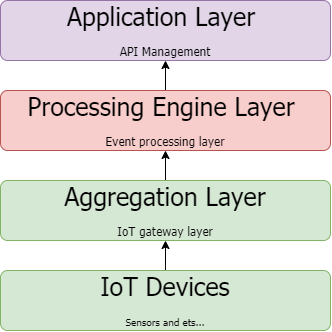
\includegraphics[scale=.5]{img/tblArtLevel.png}}
	\caption{معماری اینترنت اشیا}
	\label{fig}
\end{figure}

برای درک بهتر، خوب است که تصویر معماری همراه با فناوری، زیر را مشاهده کنید:

\begin{figure}[htbp]
	\centerline{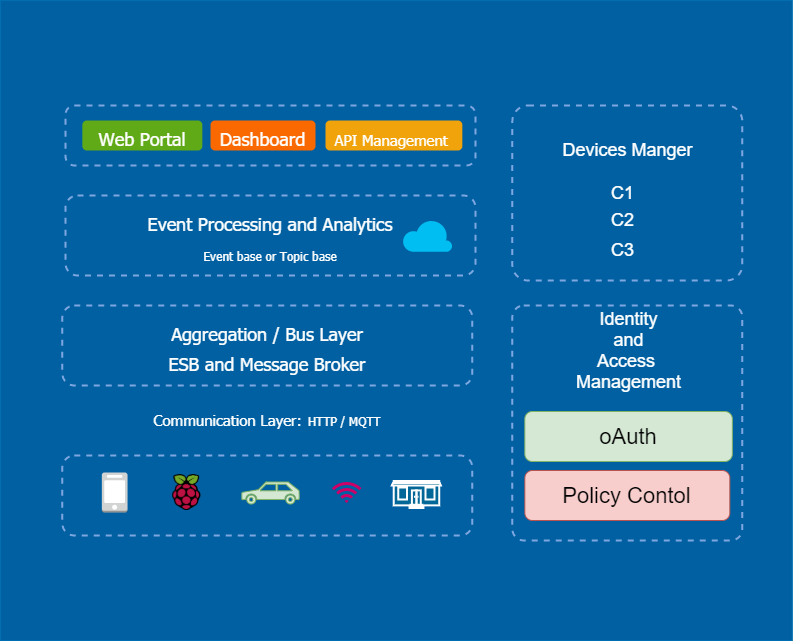
\includegraphics[width=250pt]{img/IoTArti-Applicability}}
	\caption{معماری کاربردی اینترنت اشیا}
	\label{fig}
\end{figure}

باتوجه به لایه های بالا، بطور کاربردی و واضع به توضیح وظیفه هر کدام از لایه ها می پردازیم. در لایه اول دستگاه هایی هستند که قدرت گرفتن اطلاعاتی مانند، گرما، سرما، رطوبت، بخار، دود سیگار، فشار خون، سیگنال های مختلف و غیره، را دارند. بعد از ورود دیتا، بوسیله پروتکل MQTT یا HTTP، با یک نام مخصوص به سمت سرور Publish میشوند، در لایه بعدی، این داده ها گرفته میشوند و همچنین در این حین سنسور های لایه اول میتوانند اطلاعات خود را بروز یا حذف کنند، در این میان لایه جاری Aggregation داده ها باهم در زمان های مختلف مقایسه کرده تا بتواند تشخیص دهد کدام داده به تازگی تغییر کرده، تا آخرین تغییرات را به لایه بعدی هدایت کند. در لایه بعدی Processing Event، براساس یکسری از محاسبتی که صورت میگیرد، داده های شما بر روی Cloud یا (اینترنت) به صورت سراسری فرستاده میشود تا شما بتوانید تمام اطلاعات دستگاه خود از طریق آدرسی مخصوص دریافت کنید، بعد از این فرایند مهم که دائما در حال تغییر، حذف و اضافه شدن است، یک (نهایتا) endpoint Wi-Fi به شما میدهد، تا کاربران بتوانند از طریق آن SSID Wi-Fi به آن متصل شوند، تا در نهایت این متصل شدن وارد پنل (داشبورد) خود شده و اطلاعات را به صورت بلادرنگ 
\LTRfootnote{RealTime Communications.}
مشاهده کننده.

قضیه این 4 لایه تمام است اما ممکن است بپرسید امنیت آن چقدر است؟\\
جواب: امنیت آن به اندازی کافی خوب است.\\

شما در نظر داشته باشید چند کلاینت میخواهند به پرتال سیستم اینترنت اشیا شما متصل شوند، هر کدام از این کلاینت ها به یک Wi-Fi endpoint متصل خواهند شد، این مسیر در ابتدا توسط شما مشخص شده که امنیت آن کم یا زیاد
\LTRfootnote{TKIP and AES}
 باشد، پس این مسئله اول\\
 
 ثانیا شما برای ورود به پنل اصلی سیستم خود توسط همان برنامه های اولیه مشخص کرده اید که با چه چیز عملیات AAA صورت گیرد، مثلا مرحله اول که Authentication است شما مشخص کردید که با ایمیل و گذرواژه خود قصد ورود را دارید یا اینکه از یکی از حساب های فیسبوک یا اینستاگرام خود استفاده میکنید؟ برای این امر شما میتوانیداز Standard Authentication Open
یا به اختصار OAuth استفاده کنید، یا اینکه توسط خود پنل اصلی یکسری پالسی ها و قوانینی برای ورود و احراز هویت داشبرد خود، به صورت آماده تعریف کنید. پس بطور کلی در این لنداسکیپ ما دو چیز خیلی مهم را داریم، اولی 
Manager Device
و دیگیری
Management Access and Identity
که در این متن توضیح داده شد.









\end{document}